\chapter{}

Рассматривали ИППН, классификацию ИППН, классификация в основном по квадрантам. Рассматривали
одно-квадрантные,двух-квадрантные, четырех-квадрантные.

\begin{circuitikz}\draw
%  (0,2)to[short,o-](1,2)
  (1.5,2) node[nigbt,rotate=90](nigbt1){}
  (1.5,2) node[above] {VT}
  (0,2)to[short,o-] (nigbt1.C)
  (nigbt1.E)-- (3,2)to[L,-o](5,2)
(0,0)to[short,o-o](5,0)
(3,0)to[Do,l_=$VD$,*-*](3,2)
  ;\end{circuitikz}

Замечание: может стоять IGBT-транзистор, может стоять мосфет,
\begin{circuitikz}\draw
  (0,0)node[nigfete](nigfete){}
  (nigfete.B) node[anchor=west] { подложка}
  (nigfete.G) node[anchor=east] {затвор }
  (nigfete.D) node[anchor=south] {сток}
  (nigfete.S) node[anchor=north] {исток}
;\end{circuitikz}

а может стоять обычный тиристор с углом искуственной коммутации:  

\begin{circuitikz}\draw
  (0,5)to[short,o-*](1,5)--(1,3)to[C,v_>=$ $](2.5,3)
  (1,3)to[C,v^<=$ $](2.5,3)--(3,3)to[Do,*-*](3,5)
  (1,5)to[Ty](3,5)--(4.5,5)to[L](4.5,4)to[Do](4.5,3)--(3,3)
  (4.5,5)--(6,5)
  (0,0)to[short,o-*](6,0)to[Do,*-*](6,5)--(8,5)to[L,l=$L_\textcyrillic{н}$](8,3.5)
  to[R,l=$R_\textcyrillic{н}$](8,2)
  (8,1)circle(0.35)
  (8.35,1)node[right]{$E_\textcyrillic{н}$}
  (6,0)--(8,0)--(8,0.65)
  (8,1.35)--(8,2);
  \draw[thin,<-] (1.75,2.6) -- (1.75,2) node[below]{должен зарядиться так};
  \draw[thin,<-] (1.75,3.4) --(1.2,3.6) node[above]{исходный заряд};
  \draw[thin,<-] (6.3,2.5) -- (6.7,2.5) node[below,rotate=90] {оставим этот диод};
  \draw[dashed] (1.2,5)-- (1.2,6);
  \draw (1.2,6)to[short,-o](1.2,6.1)node[left] {\large{-}};
  \draw[dashed] (2.8,5)-- (2.8,6);
  \draw (2.8,6)to[short,-o](2.8,6.1)node[right] {\large{+}};
;\end{circuitikz}

Искусственная коммутация $\cong$ принудительная коммутация $\cong$ ёмкостная коммутация.
Искусственная коммутация и  принудительная коммутация -- синонимы.
\begin{circuitikz}
\begin{scope}[scale=0.75]
  \draw[dashed] (1.2,5)-- (1.2,6);
  \draw (1.2,6)to[short,-o](1.2,6.1)node[left] {\large{-}};
  \draw[dashed] (2.8,5)-- (2.8,6);
  \draw (2.8,6)to[short,-o](2.8,6.1)node[right] {\large{+}};
  \end{scope}
  ;\end{circuitikz} -- Кратковременно подключить, искусственно включить, принудительно
включить источник. Чаще всего таким источником является заряженный конденсатор. 

\begin{circuitikz}
\begin{scope}[scale=0.75]
  \draw (1.2,5)-- (1.2,6);
  \draw (1.2,6)to[short,-o](1.2,6.1)node[left] {\large{-}};
  \draw (2.8,6)to[ospst] (2.8,5);
  \draw (2.8,6)to[short,-o](2.8,6.1)node[right] {\large{+}};
  \draw[thin,red,->] (0,5.2) -- (0.4,5.2) arc(-90:0:0.2) -- (0.6,6)  
  arc(180:90:0.6)  --(2.8,6.6) node[midway,above] {ток}
  arc(90:0:0.6)-- (3.4,5.4) arc(180:270:0.2) -- (3.9,5.2);
  \end{scope}
;\end{circuitikz} -- источник перехватывает \underline{ток} нагрузки.
Но главная задача -- отключить нагрузку.

Это делается в два этапа:
\begin{itemize}
\item запереть тиристор
\item отключить нагрузку
  \end{itemize}

\begin{circuitikz}
\begin{scope}[scale=0.75] 
  \draw (0,5)-- (1.2,5)-- (1.2,6) to[C,l_=$C$](2.8,6)--(2.8,5) -- (4,5);
  \draw[thin,red,->] (0,5.2) -- (0.4,5.2) arc(-90:0:0.2) -- (0.6,6)  
  arc(180:90:0.6)  --(2.8,6.6) node[midway,above] {ток}
  arc(90:0:0.6)-- (3.4,5.4) arc(180:270:0.2) -- (3.9,5.2);
  \end{scope}
;\end{circuitikz} -- конденсатор идеально подходит для обоих этапов. Конденсатор перезаряжается
и перехватывает энергию. Ёмкостная коммутация -- частный случай искуссственной коммутации,
когда источником является конденсатор.

Можем использовать импульсный трансформатор. 

Как отключить тиристор:

\begin{circuitikz}
\draw (0,4) to[Ty-] (0,0);
	\draw (0,3.5) -- (2,3.5) to[C] (2,2) to [Ty-] (2,0.5) -- (0,0.5);
	\draw[<-] (2.25, 1.25) -- (3.25,1.25) node[right] {\begin{minipage}[t]{0.5\textwidth}вспомогательный тиристор, 
	он включается, после включения заряжается конденсатор, когда конденсатор зарядится, тиристор отключится\end{minipage}}; 
\end{circuitikz}


Латышко в 1970 году защищал кандидатскую диссертацию по автоматическому регулированию реактивной мощности. В спимке литературы
было 270 работ, часть из которых обзоры. 96 патентов
В 1970 году человечество было сконцентрировано на искусственной коммутации. Количество статей,
посвященных искуственной коммутации измерялось четырехзначными цифрами.

Пример работы схемы:

\begin{circuitikz}\draw
  (0,5)--(1,5)--(1,3)to[C,v_>=$ $](3,3)to[Ty,l=$V_{SK}$,mirror](3,5)--(4,5)
  (0,5) node[left] {+} (0,1.2) node[left] {$-$} (4,5)node[right]{+} (4,1.2)node[right]{$-$};
%  (0,1.2)--(4,1.2); зачем это было нужно?
  \draw[thin,<-] (2,2.6) -- (1.6,2.3) node[below] {\begin{tabular}{c}по щучьему веленью\\
      конденсатор заряжен так\end{tabular}};
  
  \draw[->, thin] (4.2,4.5) -- (4.2,1.5); % от плюса к минусу
  
	% рисунок справа
	\draw[thin,->,>=latex] (5.5,3) -- (10,3);
	\draw[thin,->,>=latex] (5.5,3) -- (5.5,5.5);
	\draw (6.5,3) -- (6.5,4) -- (6.8,4) -- (6.8,3); 
	\draw[dashed] (6.5,4) -- (5.5,4) node[left] {$U_\textcyrillic{п}$};
        \draw (6.8,4) -- (6.8,5);
	\draw[thin,<->] (6.5,5.2) -- (6.8,5.2) node[midway, above] {$\tau$}; 
	\draw[domain=6.8:7.5] 
	 plot ({\x},{3.98*(-1+exp(-(\x-6.8)))+5});
        \draw[<-,thin,>=latex] (6.9,4.7) --++ (2,1) node[right] {напряжение на конденсаторе};
	% 4 = 3.98*(-1+exp(-(\x-6.8)))+5 
	% => exp(-(\x-6.8)) = 1 - 1/3.98   =>   -(\x-6.8) = ln(1 - 1/3.98)   =>   \x = 6.8 - ln(1 - 1/3.98) = 6.8 + 0.29 = 7.09
	\newcommand{\x}{7.09}
	\draw[thin] (\x, {3.98*(-1+exp(-(\x-6.8)))+5}) -- (\x,3);
	\draw[thin, <-,>=latex] (\x-0.03,3-0.03) --++ (-0.5,-0.25) node[below] {$t$ отпирания};
	%3 = 3.98*(-1+exp(-(\x-6.8)))+5
	% => exp(-(\x-6.8)) = 2 - 1/3.98 => \x = 6.8 - ln(2 - 1/3.98) = 7.36
	\renewcommand{\x}{7.36}
	\draw[thin, <-,>=latex] (\x+0.15,3-0.03) --++ (0.3,-0.7) node[below right] {$t$ выключения};
	\draw[thin, <->] (6.6, 4) -- (6.6,5);
	\draw[thin, <-]  (6.6+0.03, 4.5) --++ (1,0) node[right] {$U_C$ начальное};

	\draw (5,1.5) node[below right] {\begin{minipage}[t]{0.6\textwidth} $\delta t > t_\textcyrillic{выключения}$ 
	-- условие успешного завершения емкостной коммутации\end{minipage}};

	\draw (0,0.5) -- (1,0.5) -- (1,-0.5) to[C] (3,-0.5) -- (3,0.5) -- (4,0.5);
	% стрелка
	\draw[red,->,>=latex] (0,0) -- (0.25,0) arc(90:0:0.25) -- (0.5,-1) arc (180:270:0.25) -- (1,-1.25) -- (3.25,-1.25) 
	arc (-90:0:0.25) -- (3.5,-0.25) arc(180:90:0.25) -- (4,0);
  
	\draw(5,-0.5) node[right] {${\displaystyle C = \frac{\Delta q}{\Delta U} = \frac{I\Delta t}{\Delta U}}$};
	\draw(5,-1.5) node[right] {${\displaystyle \Delta U  = \frac{I}{C}\Delta t}$};


	\draw (0,-2.2) node[right] {стало так};
	\draw (0,-2.5) -- (1,-2.5) -- (1,-3.5) to[C] (3,-3.5) -- (3,-2.5) -- (4,-2.5);
	\draw (1.5,-3.2) node {$+$}  (2.5,-3.2) node {$-$} ;
	% стрелка
        \draw[red,->,>=latex] (0,-3) -- (0.25,-3) arc(90:0:0.25) -- (0.5,-4) arc (180:270:0.25) -- (1,-4.25) -- (3.25,-4.25)
        arc (-90:0:0.25) -- (3.5,-3.25) arc(180:90:0.25) -- (4,-3);

	% большая стрелка y=-3.2
	\draw (4.5,-3) -- (5.5,-3) -- (5.5,-2.8) -- (5.9,-3.2) -- (5.5,-3.6) -- (5.5,-3.4) -- (4.5,-3.4);


	\draw (6.3,-2.2) -- (8.3,-2.2);
	\draw ({6.8}, -4.2) to[Ty-] ({6.8}, -2.2);
	\draw (7.8,-2.2) to[L, l={$L_k$}] (7.8,-3.2) to[D-,l={VD2}] (7.8,-4.2) node[below]
	{\begin{minipage}[t]{0.45\textwidth}отпирается диод -- и в этот момент отключаетя сам\end{minipage}};

\end{circuitikz}

Как по щучьему веленью. В первый раз открываем $VS_{k}$. В момент, когда я отпираю $V_S$:

\begin{tikzpicture} 
	\draw (0,1) node[above] {тиристор включил два контура};
	\draw (0,0) ellipse (2 and 1);
	\draw (-0.5,1) to[Ty-] (0.5,1); \draw  (-0.5,-1) to[C] (0.5,-1);
	\draw (1.3,0.8) to[L] (1.8,0.2) (1.8,-0.2) to[D-] (1.3,-0.8); 

	\draw (5,0) ellipse (1.4 and 1);
	\draw (6.35,0.4) to[L,l={${\displaystyle \frac{LI^2}{2}}$}] (6.35,-0.4);
	\draw (4.5,-0.9) to[C] (5.5,-0.9);
	\draw (7.5,0.1) node[right] {\begin{minipage}[t]{0.27\textwidth} -- Энергия поля. \\ в этом контуре ток перезаряжает\end{minipage}};
	\path[->] (6.5,-0.4) edge[bend left=30] node[below right] {энергия вернулась в конденсатор} (5.2,-1.2);
\end{tikzpicture}

Диод $VD2$ прекращает колебания. При включении включается $V_{SK}$. При этом конденсатор $C$ проводит ток
от $U_\textcyrillic{П}$ в нагрузку и заряжается полярностью в  кружке 
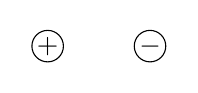
\begin{tikzpicture}
	\draw (0,0) circle(0.2) node {$+$}  (1.3,0) circle(0.2) node {$-$};
\end{tikzpicture}. 
Процесс заряда завершается, когда $U_C$ сравняется с $U_\textcyrillic{П}$ и откроется диод $V_{D1}$.
В дальнейшемм при отпирании $V_S$ и приложении в нагрузке $U_\textcyrillic{П}$ начинает протекать ток
по контуру колебательной цепи $V_S - L_K - V_{D2} - C$. Конденсатор разряжается и перезаряжается за одну
полуволну резонансной частоты контура. Конденсатор оказывается заряжен нужной для $U_K$ полярностью 
и величиной напряжения близкой к $U_\textcyrillic{П}$.
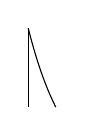
\begin{tikzpicture}[scale=0.5]
\draw (6.8,3) -- (6.8,5);
       \draw[domain=6.8:7.5]
         plot ({\x},{3.98*(-1+exp(-(\x-6.8)))+5});
\end{tikzpicture} -- иголка примерно равна $U_\textcyrillic{П}$.

Чем хороша  -- позволяет использовать обычные тиристоры. Плоха $\delta t > t_\textcyrillic{выкл}$. Тиристоры
нужны быстродействующие.

\begin{tikzpicture}
\draw (0,0) node[right] {$\displaystyle \delta t = U_C \sim \frac{U_\textcyrillic{П}}{I_{max}}$}; 
\draw[<-,>=latex] (2.6,0.3) --++ (0.5,0.25) node[right] {(меньше из-за КПД 95,98 \%) $<U_\textcyrillic{П}$}; 
\draw[<-,>=latex] (2.8,-0.3) --++ (0.5,-0.25) node[right] {условие должно выполнятся для тока перегрузки}; 
\end{tikzpicture}

Условие $< U_\textcyrillic{П}$ -- ерунда. $I_{max}$ -- это критично.

\begin{tikzpicture}
\draw (0,0) node[right] {$\displaystyle C \geqslant K\frac{t_\textcyrillic{выкл}I_{max}}{U_C < U_\textcyrillic{П}}$}; 
\draw[<-,>=latex] (1,-0.2) --++ (0,-0.5) node[below] {K -- коэффициент запаса $>1 (1.2, 1.5,2)$}; 
\end{tikzpicture}

Выбирали на максимальный ток, а работаю при минимальной, ток Х.Х. Наклон $\sim$ току 
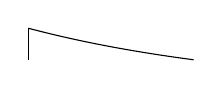
\begin{tikzpicture}[yscale=0.2,xscale=3]
\draw (6.8,3) -- (6.8,5);
       \draw[domain=6.8:7.5]
         plot ({\x},{3.98*(-1+exp(-(\x-6.8)))+5});
\end{tikzpicture}

Схема может не работать при малых токах.

\begin{tikzpicture}
\draw (0,0) to[C] (1.5,0) to[L] (1.5,-1.5) -- (0,-1.5) to[D-] (0,0);
\draw[<-,>=latex] (1.7,-0.75) --++(1,0) node[right] {ускоряет перезагрузку конденсатора};
\end{tikzpicture}

Надежность схемы снижается.

Последнее уточнение к схеме ... похожи на выпрямители. По аналигии с выпрямителями ИППН могут быть многофазными.
Делаются для уменьшения пульсаций. Подключаются а разным 
\begin{tikzpicture}
	\draw (0,0) to[C,l_={$U_\textcyrillic{П}$}] (0,-1);
\end{tikzpicture}

подключаются с разными фазами.
